\section{Introduction}
%BASED ON PRELIMIANARY RESEARCH, TOOLS SHOULD BE DEVELOPED WITH A MODULAR MINDSET AND ALLOW FOR TWEAKABLE PARAMTERS and stuff

%Describe basic concept of the product (context)
%We have a collaboration with TAW
%They make 3D point n click game
%Framing system
%Path system

\begin{figure*}[t]
\centering
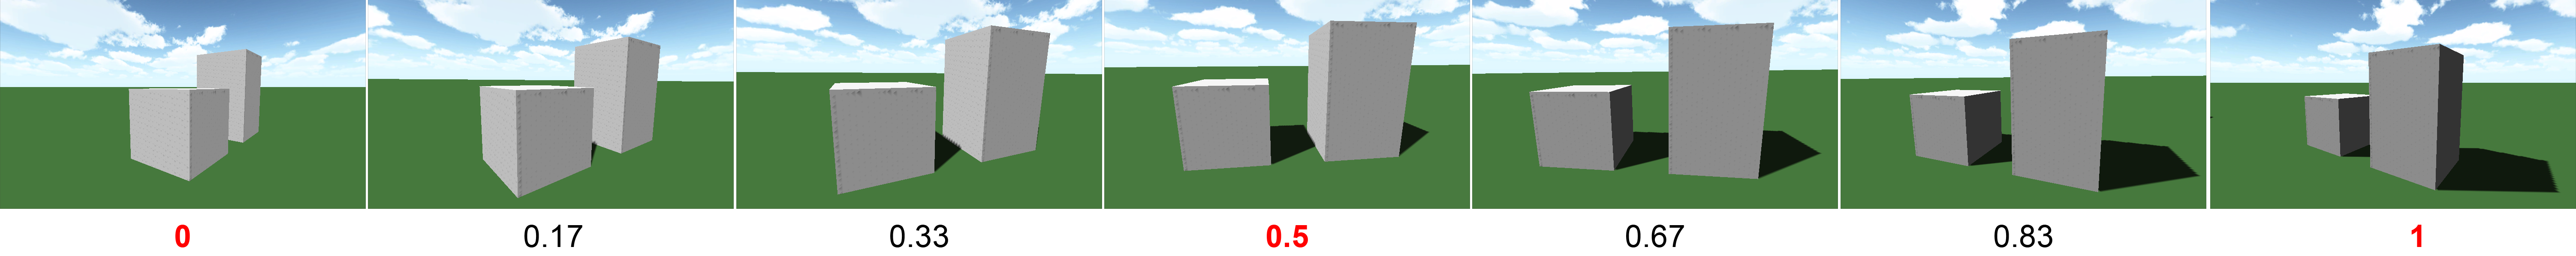
\includegraphics[width=1\textwidth]{Pics/Interpolation}
\caption{The test participant used had two monitors at his disposal while working with the tool.}
\label{fig:Interpolation}
\end{figure*}

There are many ways to design camera motions in games. Fundamentally, one can distinguish between \textit{cinematic sequences} and \textit{interactive gameplay}. These two are typically considered mutually exclusive, because cinematic sequences per definition is non-interactive \cite{haigh-hutchinson_real-time_2009}. However, it is also possible to mix those two, so the camera can dynamically adapt to certain things happening in the game like game events and player input. This means that a sequence does not have to be viewed in exactly the same way every time. 

This present paper will present an approach to create a tool for a specific group of artists. The tool will be able to define camera movements in a game where the player avatar can only move along predefined paths. Creating a tool for these artists is challenging since they have knowledge and experience working in the time domain (animation), whereas the game will be dynamic and interactive. The created camera tool, named \textit{Framing-based Camera Tool} (FCT), will be designed together with these artists.

%Games often require the ability to replay previous sequences of the gameplay. This can be used to replicate certain events to re-create the motion and visual state of objects in a scene \cite{haigh-hutchinson_real-time_2009}. This can be achieved by recording the rendering state of objects on a set amount of frames, and then use \textit{interpolation} to calculate the state of said objects. Interpolation is a method of inserting intermediate values into a set of data and makes it possible to take sampled data and generate new points in between \cite{haigh-hutchinson_real-time_2009}. Replaying of this data can be referred to as \textit{keyframing}. Keyframing of camera data requires position and orientation of the camera, together with a time interval between the samples \cite{haigh-hutchinson_real-time_2009}.

The outline of the paper is as follows. We will discuss the related work in the next section. In Section 3 we will describe how the artists was used to help create the final design of FCT. Section 4 we present FCT while Section (5?) will show how we evaluated FCT and its results. We end by with a summary and future work in Section (6?).

%During the collaboration, it was decided that we should focus on developing a camera system for the game. This tool should empower the artists, so that the artists didn't have to worry about technical details. It should be simple to set up and function in a similar fashion as other 3D applications that the TAW students have been trained in during their three-year education. The camera tool was chosen, since it does not directly influence and interfere with the gameplay, making it easier for the other programmers to work directly on the game.

%Before we began designing and implementing the tool, we conducted several preliminary studies to get an understanding of how game development tools should be made. We visited two game companies (KnapNok Games and Unity Studios), as well as conducting an online survey to gather, information about game development tools. The key findings were that the tool should be developed in a modular fashion and allow the user to tweak as many parameters as deemed necessary. Additional notes from the studies can be found in \textbf{APPENDIX X}.



%Sometimes it might be necessary to put certain restrictions on where the player can move. An example of this could be a special "boss battle" where the player is confined in a restricted area. Typically, the camera would zoom out and focus on specific parts of this boss enemy (e.g. a weak point). The camera dynamically frames the scene in such a way so that the player and the enemy are visible at all times \cite{haigh-hutchinson_real-time_2009}.

%This project is based on a collaboration between Medialogy and a group of artists from The Animation Workshop (TAW) in Viborg. As their bachelor project, the students at TAW developed a 3D point 'n click game, \textit{FEELS}, for the iPad using the Unity game engine. The TAW project spanned two semesters (pre-production and production), whereas this Medialogy project lasted only the first semester. Two additional programmers have also been working full-time on the project.